\documentclass [a4paper,12pt,oneside,final]{article}
\usepackage[left=15mm,top=15mm,right=15mm,bottom=20mm]{geometry}
\usepackage{tikz}
\usepackage{float}
\usetikzlibrary{arrows,positioning,shapes.geometric}

\title{%
Redes Neuronales \\
Análisis del modelo Integrate-and-Fire \\*[23pt]
Trabajo Práctico 2 \\
}
\date{2020}
\author{Igor Andruskiewitsch}

\begin{document}
    \maketitle

\section{Introducción}

Este trabajo está orientado a comprender el modelo {\bf Integrate-and-Fire}, que modela la evolución temporal del potencial de membrana $ V_m(t) $ en el tiempo $ t $, entre el interior y el exterior de una neurona genérica. Descrito por la siguiente ecuación diferencial ordinaria (ODE):

\[ \dot{V}_m(t) = {1 \over \tau_m} (E_L - V_m(t) + R_m I_e(t)) \]

Donde:

\begin{itemize}
    \item {$ E_L $ es el potencial en reposo ($mV$) }
    \item {$ I_e(t) $ es la corriente eléctrica externa inyectada en el tiempo $ t $ ($mV$) }
    \item {$ R_m $ es la resistencia en megaOhms ($ M\Omega $) }
    \item {$ \tau_m $ es el tiempo característico de la membrana }
\end{itemize}

\section{Resolución}

\subsection{Resolución analítica}

Si consideramos la corriente externa como una constante $ I_e(t) = I_e $, podemos buscar una solución analítica a nuestro modelo. Consideramos los siguientes valores para los parámetros:

\[ V_m(t = 0) = E_L = -65 \ mV, \qquad R = 10 \ M\Omega, \]
\[ \qquad V_{th} = -50 \  mV, \qquad \tau_m = 10 \ ms, \qquad I_e = 2 \  nA \]

Teniendo en cuenta que ahora $ I_e $ es una constante, podemos reescribir la ecuación de la siguiente forma:

\[ \dot{V}_m(t) = {1 \over \tau_m} (E_L - V_m(t) + R_m I_e(t)) = A V_m(t) + B \]

Donde: $ \, A = { {- 1} \over \tau_m }, \, B = { {R_m I_e + E_L} \over \tau_m } $.


\pagebreak
Luego, despejando:

\[ V'(t) = A V(t) + B  \Rightarrow { V'(t) \over {A V(t) + B} } = 1 \]

Hacemos el reemplazo $ U(t) = A V(t) + B $, $ U'(t) = A V'(t) $, luego:

\[ V'(t) = { U'(t) \over A } \Rightarrow { U'(t) \over A U(t) } = 1 \Rightarrow { U'(t) \over U(t) } = A \Rightarrow { \int {U'(t) \over U(t)} dt } = \int { A \  dt }\]

Ahora, sabiendo que $ \int { {f'(x) \over f(x)} dx } = \ln (f(x)) + C_0  $ y $ \int A \ dx = Ax + C_1 $, podemos resolver ambas integrales: $ \ln (U(t)) = A t + C $ donde C es constante. Luego:

\[ \ln (U(t)) = A t + C  \Rightarrow U(t) = e^{A t + C} = A V(t) + B \]
\[ \Rightarrow V(t) = {1 \over A} ( e^{At + C} - B ) = ({ e^C \over A }e^{At}) - { B \over A } \]

Tomando la constante $ k = { e^C \over A } $ y reemplazando $ A $ y $ B $ obtenemos:

\[ k e^{-t \over \tau_m } - { {( R_m I_e + E_L ) \over \tau_m } \over {-1 \over \tau_m } } = k e^{-t \over \tau_m } + R_m I_e + E_L \]

Ahora necesitamos conocer el valor de $ k $. Esto lo podemos hacer ya que conocemos el valor inicial en $ t = 0 $:

\[ V_m(t = 0) = k e^{ -t \over \tau_m } + R_m I_e + E_L = -65 \Rightarrow k = - R_m I_e \]

Reemplazando, obtenemos:

\[ V_m(t) = (- R_m I_e) e^{-t \over \tau_m} + R_m I_e + E_L = (R_m I_e) (- e^{-t \over \tau_m} + 1) + E_L \]

Al graficar esta fórmula para los valores de $t$: $ 0 \ ms \leq t \leq 200 \ ms $ y los parámetros antes mencionados obtenemos la siguiente curva:

\begin{figure}[ht]
  \centering
  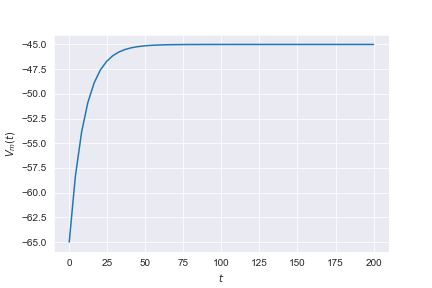
\includegraphics[width=10cm,keepaspectratio]{./diagramas/grafico_a.png}
  \caption{Solución analítica sin umbral de disparo}
\end{figure}

\pagebreak
\subsection{Aproximación con Runge-Kutta de 4to orden}

En esta sección, vamos a comparar los resultados dados por la resolución analítica sin considerar el umbral de disparo, con los resultados dados por la aproximación usando Runge-Kutta-4 (RK4), incluyendo el umbral de disparo. Ambos se realizan utilizando $ 0 \ ms \leq t \leq 200 \ ms $ y el caso de RK4 con un paso de integración $ h = 0.05 \ ms $.

\begin{figure}[ht]
  \centering
  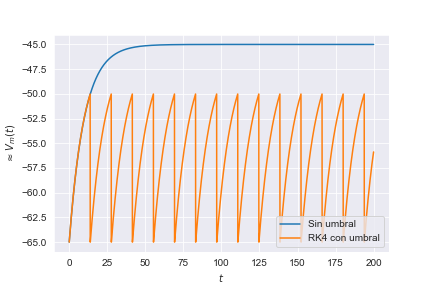
\includegraphics[width=10cm,keepaspectratio]{./diagramas/grafico_b.png}
  \caption{Comparación entre solución analítica sin umbral de disparo y aproximación con RK4 con umbral de disparo en $-50 \ mV$}
\end{figure}

Podemos observar que ambos métodos comienzan con una crecida exponencial y mientras que uno se estabiliza, el otro vuelve a realizar el mismo proceso ya que vuelve al valor inicial. Esto se debe a que en el primer gráfico no incluimos el {\it umbral de disparo}. 

\section{Comprensión de $I_e$}

En esta sección vamos a realizar algunos experimentos para comprender la importancia del {\bf input} $I_e$ en el modelo. Vamos a comenzar por intentar entender la relación entre $I_e$ y la frecuencia del disparo variando con $ 0 \leq I_e \leq 50  $:

\begin{figure}[ht]
  \centering
  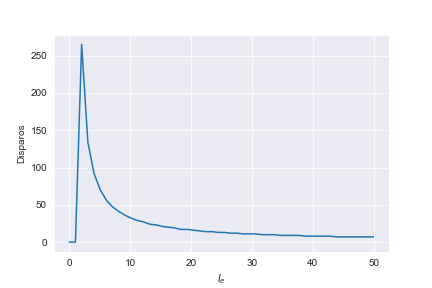
\includegraphics[width=11cm,keepaspectratio]{./diagramas/grafico_c.png}
  \caption{Relación entre $I_e$ y la frecuencia de disparo}\label{fig:c}
\end{figure}

Como podemos observar en la figura \ref{fig:c}, para los casos $I_e = 0$ y $I_e = 1$ no hay ningún disparo y por lo tanto su frecuencia es 0. Sin embargo, para $I_e = 2$ ya obtenemos disparos y a medida que $I_e$ incrementa tenemos una frecuencia cada vez más alta. La frecuencia graficada corresponde a la {\bf cantidad de disparos} que sucedieron en el rango $ 0 \ ms \leq t \leq 200 \ ms$.

\subsection{Variando $I_e$ de manera uniforme}

Al comienzo habíamos definido el $I_e(t)$ como una función que depende de $t$, luego, para poder encontrar una solución analítica pasamos a tomar $I_e(t) = I_e$ como una constante. Ahora vamos a variar a $I_e$ de manera uniforme entre $0$ y $5$ para cada $t$, para ver cómo se comporta el modelo:

\begin{figure}[ht]
  \centering
  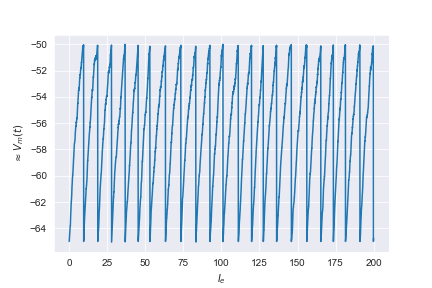
\includegraphics[width=11cm,keepaspectratio]{./diagramas/grafico_d.png}
  \caption{Aproximación del modelo con $I_e$ uniformemente distribuido}\label{fig:d}
\end{figure}

En la figura \ref{fig:d} podemos observar que aún variando uniformemente el valor de $I_e$ en función de $t$, seguimos viendo {\it picos}, y a una frecuencia similar a la que obtuvimos con $I_e = 2$. Otra observación que surge a partir del gráfico son las formas de las líneas que reflejan el flujo de entrada discontinuo.

\section{Conclusión}

Se logró obtener una solución analítica del modelo {\bf Integrate-and-Fire} al tomar $ I_e(t) = I_e $ constante, que produjo un gráfico exponencial. Por otro lado también vimos que al aproximar con RK4 obteníamos valores muy parecidos a los dados por la resolución analítica y pudimos comenzar a probar el umbral de disparo. Por último, sabiendo que la implementación de RK4 es lo suficientemente buena para ver el comportamiento del modelo, pudimos utilizar $ I_e(t) $ dependiente de $t$ y vimos que aún así el modelo mantenía un comportamiento parecido al visto en los gráficos anteriores.

\end{document}
